	
	Les actions sont exécutées à chaque pas de temps (\textit{tick}) et sur le \textit{patch} où se situe l'agent au moment de leur exécution.
	
	\textit{Remarque : il existe cependant une action logique L\_Instant qui permet d'exécuter plusieurs actions en un seul tick.}
	
	Les actions se spécialisent en actions proprement dites (préfixe A) ainsi qu'en actions logiques (préfixe L) qui regroupent des actions et d'autres actions logiques (cf. Figure \ref{HA}).
	
	\begin{figure}[!h]
	\begin{center}
	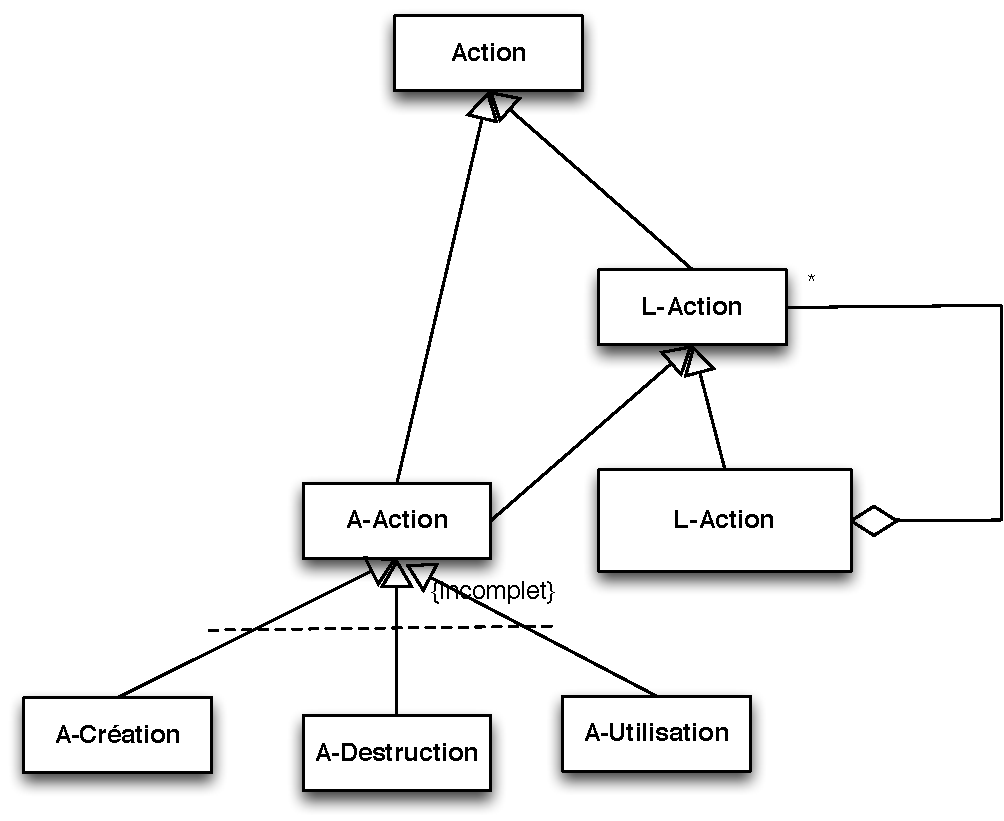
\includegraphics[scale=0.5]{DocumentationActions/HA.pdf}
	\caption[HA]{Hiérarchie des actions \\}
	\label{HA}
	\end{center}
	\end{figure}
\newpage
\section{Les actions A}
	\subsection{Les actions relatives aux objets}
	\subsubsection{A\_CreateObject} 

% modification complète de Changed Object en Modified Object

Cette action crée un objet conformément au processus de fabrication (recette ou \textit{recipe}) défini au préalable. 

La signature de l'action  est A\_CreateObject(Created Object) :
	\begin{itemize}
	\item \texttt{Created Object}, est l'objet à fabriquer.
	\end{itemize}
	
Exemple (pour un agent agriculteur) A\_CreateObject(Houe) lance la recette de fabrication de la Houe qui nécessite un bâton pour le manche et un soc (pièce métallique).
	%Cette action permet a l'agent de fabriquer un objet a partir d'autres objets présents dans son inventaire. 
	Si l'agent ne possède pas les deux objets requis pour fabriquer la houe l'action ne fera rien, sinon, elle fabriquera 1 unité de cet objet et l'ajoutera à l'inventaire de l'agent exécutant l'action. Les objets élémentaires ayant servi à la fabrication seront supprimés de l'inventaire.

\subsubsection{A\_AddObject}
Action permettant d'ajouter N objets à l'inventaire de l'agent.  

La signature de l'action est A\_AddObject(Modified Object, N) :
	\begin{itemize}
	\item \texttt{Modified Object}, précise le type d'objet utilisé pour créer directement l'objet à ajouter à l'inventaire de l'agent (sans utiliser la recette)
	\item \texttt{N}, le nombre d'objets à ajouter.
	\end{itemize}
	
	
\subsubsection{A\_DropObject}  
Action permettant de supprimer N objets de l'inventaire de l'agent.  

La signature de l'action est A\_DropItem(Modified Object, N) :	
	
	\begin{itemize}
	\item \texttt{Modified Object}, type de l'objet à retirer de l'inventaire de l'agent,
	\item \texttt{N}, le nombre d'objets à retirer.
	\end{itemize}
	
\subsubsection{A\_Transform} 

Cette action transforme une ressource prélévée sur un patch en objet.

La signature de l'action est A\_Transform (Resource to Collect, Modified Object) :
%\textit{Remarque : la ressource est appelée phéromone (hérité de Turtle Kit)}

	
	\begin{itemize}
	\item \texttt{Resource to Collect}, le type de la ressource que l'agent prélève,
	\item \texttt{Changed Object}, l'objet correspondant (pour le modélisateur) à ajouter à l'inventaire de l'agent.
	\end{itemize}
	
Exemple : un agent exécute 	 A\_Transform (Blé, Meule).

\subsubsection{A\_UseObject}
Cette action correspond à l'usage d'un objet. 


La signature de l'action est A\_UseObject(Modified Object, N) :
	\begin{itemize}
	\item \texttt{Modified Object}, le type d'objet à utiliser,
	\item \texttt{N}, le nombre.
	\end{itemize}
	
		
\subsubsection{A\_AddObjectXCogniton}

La signature de l'action est A\_AddObjectXCogniton(Modified Object, variation,base, Cogniton) :
\begin{itemize}
	\item \texttt{Modified object}, le type d'objet à ajouter,
	\item \texttt{variation}, la variation du nombre d'objets à ajouter,
	\item \texttt{base}, le nombre d'objets à ajouter par défaut,
	\item \texttt{Cogniton}, le cogniton référence.
	\end{itemize}
	
Cette action, suite à l'existence d'un Cogniton dans l'esprit de l'agent, ajoute  des objets à l'inventaire de l'agent en fonction de paramètres contextuel :
\begin{itemize}
\item  si le cogniton n'existe pas dans l'esprit de l'agent, l'action ajoute  \textit{base} objets à l'inventaire,
 \item si le cogniton existe dans l'esprit de l'agent, l'action ajoute \textit{base} + (\textit{variation} * poids de \textit{Cogniton}) objets à l'inventaire.
 \end{itemize}
	

Exemple  : un agent qui possède le Cogniton Artisan avec un poids de 2,  exécute l'action
A\_AddObjectXCogniton(Houe, 0.5,1, Artisan) ce qui lui permet d'ajouter 1+ 0.5*2 c'est-à-dire 2 Houes à son inventaire ; si l'agent ne possède pas le Cogniton Artisan l'exécution ajoute 1 seule Houe à son inventaire.
	
	
	
	\subsection{Les actions relatives aux aménagements}
	\subsubsection{A\_CreateFacility} 
	Cette action permet à l'agent de construit l'aménagement sur le patch où il se trouve au moment de l'exécution ; la signature de l'action est A\_CreateFacility(Facility) :

	\begin{itemize}
	\item \texttt{Facility}, le type d'aménagement à construire
	\end{itemize}
	
	
\subsubsection{A\_EraseFacility} 
Cette action permet à l'agent de détruire l'aménagement du  patch où il se trouve au moment de l'exécution, la signature de l'action est A\_EraseFacility(Facility) :

	\begin{itemize}
	\item \texttt{Facility}, le type d'aménagement à détruire
	\end{itemize}
	

\subsubsection{A\_GoToFacility} 
Cette action permet à l'agent d'atteindre le patch le plus proche disposant de l'aménagement (si celui ci existe) , la signature de l'action est A\_GoToAmenagement(Facility) :
	\begin{itemize}
	\item \texttt{Facility}, le type d'aménagement à cibler
	\end{itemize}
	
	.
	
\subsubsection{A\_UseFacility} 
Cette action permet à l'agent l'usage de l'aménagement (à condition qu'il soit sur le patch sur lequel se trouve l'agent), la signature de l'action est A\_UseAmenagement(Facility) :
	\begin{itemize}
	\item \texttt{Facility}, le type d'aménagement à utiliser
	\end{itemize}
	
\subsubsection{A\_DepositObjectInAmenagementLargeQuantity}

L'action permet de déposer N objets 	dans un aménagement d'un agent du groupe si l'on se trouve sur l'aménagement en question. 
La signature de l'action est A\_DepositObjectInAmenagementLargeQuantity(Modified Object, N) :
\begin{itemize}
\item Modified Object, type de l'objet à déposer dans l'aménagement.
\item N, le nombre d'objets à déposer.
\end{itemize}

\subsubsection{A\_withdrawObjectInAmenagementLargeQuantity}

L'action permet de retirer N objets dans un aménagement d'un agent du groupe si l'on se trouve sur l'aménagement en question. 
La signature de l'action est A\_withdrawObjectInAmenagementLargeQuantity(Modified Object, N) :
\begin{itemize}
\item Modified Object, type de l'objet à retirer de l'aménagement.
\item N, le nombre d'objets à retirer.
\end{itemize}

\subsubsection{A\_withdrawObjectInAmenagementHereLargeQuantity}

L'action permet de retirer N objets dans un aménagement d'un agent si l'on se trouve sur l'aménagement en question. 
La signature de l'action est A\_withdrawObjectInAmenagementHereLargeQuantity(Modified Object, N) :
\begin{itemize}
\item Modified Object, type de l'objet à retirer de l'aménagement.
\item N, le nombre d'objets à retirer.
\end{itemize}

	
	\subsection{Les actions relatives aux cognitons}
	\input{DocumentationActions/ActionsCognitons}
	
	\subsection{Les actions relatives aux déplacements}
		\subsubsection{A\_MoveTowards}  
	
	L'action permet à l'agent de se déplacer vers une cible spécifiée.
	
	\textit{Remarque : la cible aura été définie par l'action A\_GetAnotherSettlementPatch.}
	 	
 	
 	\subsubsection{A\_MoveRandomly} 
	
	L' action permet à l'agent d'effectuer un pas  dans une direction aléatoire.

\textit{Remarque : la longueur du pas dépend de la facilité de traversée du patch (cf. passability)}

	\subsubsection{A\_DoNothing}
	
	Cette action permet à l'agent de n'exécuter aucune action.
	
	\subsubsection{A\_ CreateSettlement}   
	
	Cette action permet à l'agent de se déplacer aléatoirement jusqu'à ce qu'il trouve un ensemble de patchs (les 8 patchs voisins immédiats)  dépeuplé de manière à créer un nouveau \textit{Settlement}.
	
	%\textit{Remarque : voir la terminologie }
	
	
	
	\subsubsection{A\_GetAnotherSettlementPatch}  
	
	Cette action définie la cible utilisée dans l'action A\_MoveTowards comme étant un des \textit{Settlement} pris au hasard dans l'ensemble des \textit{Settlement} existants.
	
	\subsubsection{A\_GoBackHome}
	
	Cette action permet à l'agent de se déplacer d'un pas vers son lieu de création s'il s'agit d'un des agents des peuplements initiaux, sinon vers le lieu où se trouvait l'agent qui l'a engendré.
	
	\subsubsection{A\_Move}
	
	Cette action déplace l'agent d'un pas dans une direction donnée.
	
	 La signature de cette action est A\_Move(String) :
	
	\begin{itemize}
	\item \texttt{String}, "NORTH","SOUTH","WEST","EAST" correspond à la direction que prendra  l'agent
	\end{itemize}
	
	\subsubsection{A\_SearchForResources} 
	
	Cette action permet à l'agent de rechercher autour de lui (dans son champ de vision)  la ressource passée en paramètre,  pour cela il se dirigera vers le patch le plus proche et  possédant cette ressource en quantité maximum. S'il ne trouve pas de patch contenant cette ressource, il se déplacera aléatoirement de un pas.
	
	 La signature de cette action est A\_SearchForResources(Resource To Collect) :
	
	\begin{itemize}
	\item \texttt{Resource To Collect}, correspond à la ressource recherchée.
	\end{itemize}
	
	\subsubsection{A\_SmellAndMove}
	
	Cette action permet à l'agent de chercher dans son voisinage immédiat le patch contenant la ressource passée en paramètre en plus grande quantité et de faire un pas dans sa direction. 
	
	La signature de cette action est A\_SmellAndMove(Resource To Collect) :
	
	\begin{itemize}
	\item \texttt{Resource To Collect}, correspond à la ressource recherchée.
	\end{itemize}
	
	\subsubsection{A\_GoToGroupFaicility}

Cette action ramène l'agent à un aménagement d'un des membres de son groupe.
La signature de l'action est A\_GoToGroupFaicility(Facility) :
\begin{itemize}
\item Facility, le type d'aménagement vers lequel l'agent doit se diriger.
\end{itemize}

\subsubsection{A\_GoToAmenagementInCommunity}

L'action de se rendre a l'aménagement demandé le plus proche de la civilisation. 
La signature de l'action est A\_GoToAmenagementInCommunity(Modified Object, N) :
\begin{itemize}
\item TypeAmenagement, type de l'aménagement auquel il faut se rendre.
\end{itemize}

\subsubsection{A\_FollowRoleInGroup}

L'action permet a l'agent de suivre un agent qui possède un certain rôle dans un groupe.
La signature de l'action est A\_FollowRoleInGroup(Role) :
\begin{itemize}
\item Role, de l'agent a suivre.
\end{itemize}

	\subsection{Les actions relatives aux agents}
		\subsubsection{A\_GiveBirth} 
	
	L'action permet à l'agent qui l'exécute de créer un nouvel agent sur le patch où il se situe : cet agent sera identique à ceux du peuplement initial.
	
	\subsubsection{A\_Die}
	
	L'action permet à l'agent qui l'exécute de se supprimer.
	
	\subsubsection{A\_DieIfAttributeUnderZero}
	
	L'action supprime l'agent qui l'exécute si la valeur de l'attribut (ou caractéristique) passé en paramètre descend en dessous de zéro. La signature de cette action est A\_DieIfAttributeUnderZero(attributeToCompare) :
	
	
	\begin{itemize}
	\item \texttt{attributeToCompare}, correspond à l'attribut à vérifier
	\end{itemize}	
	
	\subsubsection{A\_ChangeAttribute} 
	
	L'action modifie une caractéristique de l'agent. 
	
	La signature de l'action est A\_ChangeAttribute(Modified attribute, n) ;
	
	\begin{itemize}
	\item \texttt{Modified attribute}, correspond à la caractéristique à modifier
	\item \texttt{n}, donne la valeur à ajouter à la caractéristique
	\end{itemize}
	
	\subsubsection{A\_Trade} 
	
	L'action A\_Trade  comporte deux actions internes, elle correspond à un échange conditionnel,  car elle suppose que si après un temps fixé (\textit{turns}) l'agent n'a pas réussi à trouver un partenaire il exécute 
la deuxième action interne sinon la première.

	La signature de l'action est A\_Trade(turns, objectToGive, nObjectToGive, objectToTake, nObjectToTake, myTag, compatibleTag) ;
	
		\begin{itemize}
	\item \texttt{turns}, correspond au nombre de ticks durant lequel l'agent attend sur son patch un autre agent pour réaliser un échange,
	\item \texttt{objectToGive}  donne l'objet que l'agent échange,
	\item\texttt{nobjectToGive} correspond au nombre n d'objets à échanger,
	\item \texttt{objectToTake}  précise l'objet reçu en échange,
	\item \texttt{nobjectToTake} correspond au nombre n d'objets reçus,
	\item \texttt{mytag}, message que l'agent passe à l'attention des autres,
	\item \texttt{compatibletag} message recherché chez le partenaire échangeur potentiel.
	\end{itemize}
	
	\subsubsection{A\_TravelTrade} 
	
	L'action A\_TravelTrade  comporte deux actions internes, elle correspond à un échange conditionnel,  car elle suppose que si après un temps fixé (\textit{turns}) l'agent n'a pas réussi à trouver un partenaire il exécute la deuxième action interne sinon la première.

	La signature de l'action est A\_TravelTrade(turns, objectToGive, nObjectToGive, objectToTake, nObjectToTake, myTag, compatibleTag) ;
	
		\begin{itemize}
	\item \texttt{turns}, correspond au nombre de ticks durant lequel l'agent cherche des partenaires commerciaux dans son voisinage et se déplace vers eux,
	\item \texttt{objectToGive}  donne l'objet que l'agent échange,
	\item\texttt{nobjectToGive} correspond au nombre n d'objets à échanger,
	\item \texttt{objectToTake}  précise l'objet reçu en échange,
	\item \texttt{nobjectToTake} correspond au nombre n d'objets reçus,
	\item \texttt{mytag}, message que l'agent passe à l'attention des autres,
	\item \texttt{compatibletag} message recherché chez le partenaire échangeur potentiel.
	\end{itemize}
	
	
	\subsubsection{A\_CreateGroup}
	
	L'action permet à l'agent  de créer un groupe. 
	
	La signature de l'action  est A\_CreateGroup(GroupToCreate) : 
	
	\begin{itemize}
	\item \texttt{GroupToCreate}, donne le type du groupe à créer.
	\end{itemize}
	
	\subsubsection{A\_HireForRole}
	
	L'action permet à l'agent exécutant d'ajouter un agent présent sur le même patch que lui à son groupe . 
	
	La signature de l'action est A\_HireForRole(GroupToCreate) :
	
	\begin{itemize}
	\item \texttt{GroupToCreate}, donne  le type du groupe dans lequel  l'agent sera admis
	\end{itemize}
	
	\textit{Remarque : un agent peut appartenir à plusieurs groupes}
	
	
	\subsubsection{A\_DisbandGoup}

Cette action détruit un groupe et retire tout les membres de celui-ci
La signature de l'action est A\_DisbandGoup(Groupe) :
\begin{itemize}
\item Groupe, le nom du groupe auquel appartient l'agent qui détruit le groupe.
\end{itemize}

\subsubsection{A\_CreatedElectedGroup}

Cette action a pour but la création d'un groupe a travers un vote. Si 50\% des votants approuve la motion, alors tout les votant rejoingne le groupe dans un certain role et le demander du vote dans un autre. 
La signature de l'action est A\_CreatedElectedGroup(Role, Role, cogniton, attribut) :
\begin{itemize}
\item Role, le nom du role dont le demandeur va rejoindre.
\item Role, le nom du role dont les votant vont rejoindre.
\item cogniton, le cogniton surlequel se base le vote.
\item attribut, le nom de l'attribut qui conditionnent le vote des votant.\end{itemize}


\subsubsection{A\_HireForRole}

Cette action recrute un agent sans groupe se trouvant sur le même patch que l'agent et lui donne un rôle dans son groupe.
La signature de l'action est A\_HireForRole(Role) :
\begin{itemize}
\item Role, le rôle dans lequel le nouvel agent recruté sera affecté dans le groupe.
\end{itemize}

\subsubsection{A\_AskRandomMemberToChangeRoleForAnother}

Cette action change le rôle d'un des membre du groupe de l'agent pour un autre rôle spécifié (s'il n'est pas déjà dans ce rôle).
La signature de l'action est A\_AskRandomMemberToChangeRoleForAnother(Role):
\begin{itemize}
\item Role, le rôle vers lequel un membre du groupe se convertira.
\end{itemize}

\subsubsection{A\_BirthGroupAndRole}

Cette action ressemble à l'action A\_Birth, elle créer un nouvel agent en appelant le BirthPlan puis ajoute le nouveau membre au groupe en lui affectant un rôle.
La signature de l'action est A\_BirthGroupAndRole(Role):
\begin{itemize}
\item Role, le rôle vers lequel le nouvel agent sera affecté dans le groupe.
\end{itemize}

\subsubsection{A\_ChangeAttributeDouble}

Cette action ressemble à l'action A\_ChangeAttribute, elle permet de modifier l'attribut d'un agent en ajoutant un N (double) à la valeur de l'attribut.
La signature de l'action est A\_ChangeAttributeDouble(Modified Attribute, N):
\begin{itemize}
\item Modified Attribute, attribut de l'agent à modifier.
\item N, la valeur à ajouter à la valeur de l'attribut.
\end{itemize}

\subsubsection{A\_ChangeRoleForAnother}

Cette action change le rôle de l'agent pour un autre rôle du groupe.
La signature de l'action est A\_ChangeRoleForAnother(Role):
\begin{itemize}
\item Role, le rôle vers lequel l'agent se convertira.
\end{itemize}

\subsubsection{A\_DieAndRemoveFacilities}

Cette action fait mourir l'agent et efface tous ses aménagements.
Cette action ne possède pas d'arguments.

\subsubsection{A\_DieAndRemoveSpecificFacility}

Cette action fait mourir l'agent et n'efface qu'un type d'aménagement.
La signature de l'action est A\_DieAndRemoveSpecificFacility(Facility):
\begin{itemize}
\item Facility, le type d'aménagements supprimés à la mort de l'agent.
\end{itemize}


\subsubsection{A\_setPoissonLaw}

Cette action modifie un attribut et lui donne la valeur d'un nombre suivant un loi de poisson de paramètre $\lambda = 10$ et $n=20$ et multiplié par 5.
La signature de l'action est A\_setPoissonLaw(Modified Attribute):
\begin{itemize}
\item Modified Attribute, est l'attribut modifié.
\end{itemize}
	
\section{Les actions L}

\subsection{Tests}


La structure générale des actions logiques de type Test est :

\begin{algorithm}
\Begin{
       
    \If{ condition }
  			 { 
  		 		action interne 1 
  		 		
   			}	   
        	\Else
        	{
        		action interne 2 
        		    	
        	}
   }  
  
\end{algorithm}

\newpage
\textit{Remarque : ces actions logiques sont toutes composées de deux actions internes (qui peuvent elles-mêmes être composites).}

Les diverses actions suivantes vont préciser le type de condition.

\subsubsection{L\_CompareAttribute}
La condition porte sur la valeur d'un attribut de l'agent.

La signature de cette action est L\_CompareAttribute(attributTocompare, comparator, n) :
\begin{itemize}
	\item \texttt{attributTocompare}, est l'attribut concerné,
	\item \texttt{comparator} l'opérateur de comparaison $<$, $>$, $<=$,$ >=$,$ ==$,
	\item \texttt{n} la valeur de comparaison.
	\end{itemize}

\subsubsection{L\_CompareObject}
La condition porte sur le nombre d'objets d'un type donné possédés.

La signature de cette action est L\_CompareObject(objectTocompare, comparator, n) :
\begin{itemize}
	\item \texttt{objectTocompare}, est le type d'objet concerné,
	\item \texttt{comparator} l'opérateur de comparaison $<$, $>$, $<=$,$ >=$,$ ==$,
	\item \texttt{n} le nombre d'objets.
	\end{itemize}
\subsubsection{L\_CompareResource}
La condition porte sur la valeur de la ressource présente sur le patch où est situé  l'agent.

La signature de cette action est L\_CompareResource(resourceTocompare, comparator, n) :
\begin{itemize}
	\item \texttt{resourceTocompare}, est le type de la ressource concernée,
	\item \texttt{comparator} l'opérateur de comparaison $<$, $>$, $<=$,$ >=$,$ ==$,
	\item \texttt{n} la valeur de la ressource.
	\end{itemize}
	
	
\subsubsection{L\_IsFacilityHere}

La condition teste la présence de l'aménagement \textit{(facility)} concerné sur le patch  où est situé  l'agent.

La signature de cette action est L\_IsFacilityHere(facility) :
\begin{itemize}
	\item \texttt{facility},  le type d'aménagement testé.
	\end{itemize}	
	
\subsubsection{L\_IsAnyFacilityHere}
La condition teste la présence d'un aménagement de n'importe quel type sur le patch  où est situé  l'agent.

\subsubsection{L\_OwnFacility}

La condition teste la possession d'un aménagement donné.

La signature de cette action est L\_OwnFacility(facility) :
\begin{itemize}
	\item \texttt{facility},  le type d'aménagement testé.
	\end{itemize}	
\subsubsection{L\_OwnCogniton}
La condition teste la possession d'un cognition.

La signature de cette action est L\_OwnCogniton(cogniton) :
\begin{itemize}
	\item \texttt{cogniton},  le type de cogniton testé.
	\end{itemize}	
\subsubsection{L\_OwnObject}

La condition teste la possession d'un objet. 

La signature de cette action est L\_OwnObject(object) :
\begin{itemize}
	\item \texttt{object},  le type d'objet testé.
	\end{itemize}	

\subsubsection{L\_IsAmenagementInCommunity}

La condition porte sur la présence d'un aménagement dans la civilisation. Il s'agit de tester si ce type d'aménagement est présent.
La signature de cette action est L\_CompareAttributeToAttribute(TypeAmenagement):
\begin{itemize}
\item TypeAmenagement est le type d'aménagement attribut concerné.
\end{itemize}


\subsubsection{L\_CompareAttributeToAttribute}

La condition porte sur les valeurs de deux attributs de l'agent, elles sont comparés par un comparateur.
La signature de cette action est L\_CompareAttributeToAttribute(Attribute1, comparator, Attribute2):
\begin{itemize}
\item Attribute1 est le premier attribut concerné.
\item comparator est l'opérateur de comparaison $<, >, \leq, \geq, == $.
\item Attribute2 est le deuxième attribut concerné.
\end{itemize}

\subsubsection{L\_CompareAttributeToConstant}

La condition porte sur la valeur d'un attribut par rapport à une constante.
La signature de cette action est L\_CompareAttributeToConstant(Attribute, comparator, Constant):
\begin{itemize}
\item Attribute est l'attribut concerné.
\item comparator est l'opérateur de comparaison $<, >, \leq, \geq, == $.
\item Constant est la constante concernée.
\end{itemize}

\subsubsection{L\_CompareGroupAttributeToPopulation}

La condition porte sur un la somme des attributs des membres d'un groupe par rapport au nombre d'individus de ce groupe.
La signature de cette action est L\_CompareGroupAttributeToPopulation(Attribute, comparator):
\begin{itemize}
\item Attribute, est l'attribut de groupe à comparer.
\item comparator est l'opérateur de comparaison $<, >, \leq, \geq, == $.
\end{itemize}

%L\_CompareNombreObjets
%L\_CompareNombreObjetsInGroupAmenagement

\subsubsection{L\_CompareRoleMembers}

La condition porte sur le nombre d'individus du groupe par rapport à un nombre N.
La signature de cette action est L\_CompareRoleMembers(N, comparator):
\begin{itemize}
\item N est le nombre à comparer à la population du groupe.
\item comparator est l'opérateur de comparaison $<, >, \leq, \geq, == $.
\end{itemize}

\subsubsection{L\_IsInThatGropInThatRole}

La condition porte sur le rôle de l'agent dans son groupe.
La signature de cette action est L\_IsInThatGropInThatRole(Role):
\begin{itemize}
\item Role, le rôle à comparer avec le rôle de l'agent.
\end{itemize}


\subsection{Algorithmiques}

Ces actions logiques composites sont associées à des structures standard algorithmique.



\subsubsection{L\_Instant}

Cette action composite effectue la globalité de ses actions internes en un seul tick.



\subsubsection{L\_Random}
Cette action composite effectue une seule de ses actions internes choisie aléatoirement en un seul tick.


\subsubsection{L\_RandomPercent}

Cette action composite n'a que deux actions internes et choisit selon le pourcentage l'action interne à exécuter.

La signature de cette action est L\_RandomPercent(n) :
\begin{itemize}
	\item \texttt{n},  le pourcentage de chance qu'à l'action interne 1 de s'exécuter.
	\end{itemize}	
	
\subsubsection{L\_Repeat}
Cette action composite ne comporte qu'une action interne qu'elle va exécuter n fois en n tick.

La signature de cette action est L\_Repeat(n) :
\begin{itemize}
	\item \texttt{n},  le nombre d'itérations.
	\end{itemize}	


